\EXERCISE
یک افراز از یک عدد طبیعی، یعنی نوشتن آن به صورت مجموع یک یا چند عدد طبیعی (جمع‌وند) و بدون در نظر گرفتن ترتیب این اعداد. ثابت کنید برای هر عدد زوج مانند
$n$
تعداد افرازهای آن که هر عدد متمایز زوج بار در آن‌ها تکرار شده باشند با تعداد افرازهای
$n$
که هر جمع‌وند آن‌ها زوج باشند، برابر است. مثلا برای عدد
$8$
،
$2 + 4 + 6$
و
$1 + 1 + 2 + 2 + 3 + 3$
به ترتیب دو افراز با جمع‌وندهای زوج و جمع‌وندهایی که هر یک زوج بار تکرار شده‌اند، هستند. (راهنمایی: شکل زیر یک افراز عدد
$8$
را نشان می‌دهد.)
\begin{center}
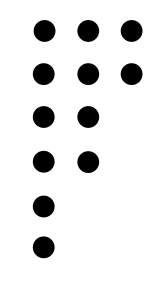
\includegraphics[height=3cm]{10.png}
\end{center}